
\pagebreak

\section*{Introduction}
\addcontentsline{toc}{section}{Introduction}



L'exercice proposé\footnote{Les livrables associés à cet exercice se trouvent à l'adresse : 
	\url{https://github.com/kad15/AF/tree/master/LIVRABLES_ATC_YUAN_BELDJILALI}} a pour finalité la modélisation et l'analyse d'un système ATC simplifié dans un cadre MBSE : Model Based System Engineering. Cette approche permet, en effet, des simulations et vérifications précoces intervenant lors de la phase décroissante du cycle en V, en amont de l'implémentation.   

\begin{figure}[H]
	\begin{center}	
		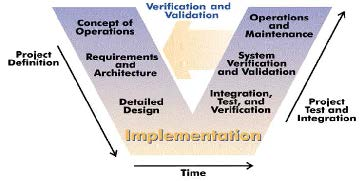
\includegraphics[scale=0.45]{images/cycleV}
		\caption{Diagramme de cycle de V\&V}
		\label{cycleV}
	\end{center}
\end{figure}

\paragraph{}
Les composants internes, constitutifs du système ATC considéré, comportent des acteurs humains, les contrôleurs, et des acteurs systèmes hardware et software. On citera les radars primaires, secondaires, les logiciels de traitement et d'affichage des données radar et de plans de vol, sans oublier les filets de sauvegarde. Le NMOC européen, Network Management Operation Centre, et le système de traitement de plan de vol national sont inclus dans le système étudié car ils participent à la fourniture du service de contrôle. Par contre, les composants humains, matériels et logiciel assurant notamment le maintien en condition opérationnelle des composants ne sont pas pris en compte dans le cadre de cet exercice.
\paragraph{}
Quant aux acteurs extérieurs, ce sont en particulier les pilotes, les compagnies aériennes, les aéronefs, le service météo. On pourrait ajouter les acteurs humains impactant la sûreté et la sécurité du système directement par le hacking du réseau ATC ou par brouillage des communications radio, par détournement de vols. Ceci impacte sur les contraintes que le système est susceptible de subir sans oublier l'acteur environnemental constitué des phénomènes météo. On choisit cependant de les ignorer également pour se focaliser sur l'objectif pédagogique principal de cet exercice qui est d'appliquer une démarche MBSE.







